\documentclass[11pt,a4paper,titlepage]{article}

\usepackage[czech]{babel}
\usepackage[utf8]{inputenc}

\usepackage[dvipdf]{graphicx}


\usepackage[bookmarksopen,colorlinks,plainpages=false,urlcolor=blue,unicode]{hyperref}
\usepackage{url}

\usepackage[left=2cm,text={17cm,24cm},top=5cm]{geometry}


\begin{document}

\begin{titlepage}

\begin{center}

\LARGE
\textsc{Vysoké učení technické v Brně \\ Fakulta informačných technológií}
\end{center}

\begin{figure}[!h]
\centering
\includegraphics[height=5cm]{img/logo.eps}
\end{figure}

\bigskip

\begin{center}
\begin{Huge}
Implementace interpretu imperativního jazyka IFJ13\\
\end{Huge}

\bigskip

\begin{Large}
Dokumentace k projektu pre předměty IFJ a IAL
\end{Large}             \\
\smallskip
\smallskip
\smallskip
Tým 013, varianta b/3/I
\end{center}

\vfill

\begin{center}
\begin{Large}
\today
\end{Large}
\end{center}

\vfill  
\begin{table}[b]

\tabcolsep=12pt
  \begin{tabular}{l c r }
Vedoucí týmu: Tomáš Bank & 19 \% & \qquad  xbankt00@stud.fit.vutbr.cz\\
&  &  \\
Mark Birger & 24 \% & \qquad \qquad \qquad \qquad \qquad  \qquad \qquad xbirge00@stud.fit.vutbr.cz\\
Roland Botka & 19 \% & xbotka00@stud.fit.vutbr.cz\\
Zdenko Brandejs & 19 \% & xbrand06@stud.fit.vutbr.cz\\
Daniil Khudiakov & 19 \% & xkhudi00@stud.fit.vutbr.cz\\
\end{tabular}

\end{table}

\end{titlepage}

\thispagestyle{empty}
\pagestyle{plain}
\pagenumbering{arabic}
\setcounter{page}{1}

\tableofcontents


\newpage
\pagestyle{plain}
\setcounter{page}{1}
\pagenumbering{arabic}




\section{Úvod} \label{uvod}	
\bigskip
	\hspace{1cm} Tento dokument popisuje návrh a implementaci interpretu imperatívního jazyka IFJ13.\\
	Varianta b/3/I udává použít pro vyhledávaní Boyer-Mooreův algoritmus (libovolný typ heurestiky), pro řazení algoritmus Shell sort a tabulku symbolů implementovánu pomocí binárního vyhledávacího stromu. \\
	 \smallskip
	\hspace{1cm}Interpret je složen ze tří hlavních částí: lexikální analyzátor, syntaktický analyzátor a interpret. Všechny tyto části jsou popsány v tomto dokumentu i se zadáním problému, jeho analýzou a popisem řešení.\\
	\smallskip
	\hspace{1cm} Dokument se skládá z několika částí. V kapitole \ref{2} je popsané zadání problému. Kapitola \ref{3} obsahuje postup naši práce. Další kapitola \ref{4} obsahuje popis řešení. Popis práce v týmu popisuje kapitola \ref{5}.	Na závěr dokumentu \ref{6} je stručné shrnutí celé práce. V kapitole \ref{7} jsou přidány přílohy obsahující strukturu konečného automatu a LL-gramatiku, protože se jedná o zásadní prvky interpretu.                   
  \bigskip


\section{Zadání problému} \label{2}
	\bigskip
	\hspace{1cm} Naším úkolem bylo vytvořit program, který načte zdrojový soubor zapsaný v jazyce IFJ13 \newline a interpretuje jej. Jestliže činnost interpretu proběhne bez chyb, vrací se návratová hodnota 0 (nula). Jestliže došlo k nějaké chybě, vrací se předem určená návratová hodnota. \\
	\smallskip
	\hspace{1cm} Jméno souboru s řídícím programem v jazyce IFJ13 bude předáno jako první a jediný parametr na příkazové řádce. Program bude přijímat vstupy ze standardního vstupu, směrovat všechny své výstupy na standardní výstup.
  \bigskip

\section{Postup práce}\label{3}
\bigskip
\hspace{1cm}Při vývoji interpretu jsme pracovali postupně. V úvodu jsme definovali seznam tokenů a navrhli jsme konečný automat. Podle konečného automatu jsme navrhli lexer a pracovali na návrhu LL-tabulky. Poté jsme implementovali  rekurzivní sestup, binární vyhledávací strom a sadu funkcí pro práci s ním. Dalším krokem bylo navrhnutí tabulky priorit operací a implementování precedenční analýzy. Implementovali jsme jednosměrný seznam instrukcí, pro který jsme navrhli instrukce. Další fází bylo generování instrukcí v parseru. Na závěr jsme začali psát interpert, popsali jsme instrukce skoku, implementovali rekurzi přes jednosměrné seznamy. Během implementace jsme opravovali chyby, které se objevily při průběžných testech. Dokumentaci jsme psali během implementace jednotlivých kroků, na závěr jsme dopsali poslední části dokumentace.
\smallskip


\section{Popis řešení}   \label{4}
\bigskip
	\hspace{1cm} V této části se zabýváme podrobnějším popisem řešení projektu. Důraz klademe na 3 hlavní části (lexikální analýza, syntaktická analýza a interpret), ale i na konečný automat, boyer-moorův algoritmus, shell sort algoritmus a tabulku symbolů.
\smallskip


\subsection{Lexikální analýza}
\bigskip

	\hspace{1cm} Je to první část interpretu. Na vstupu lexikálního analyzátoru (scanneru) je zdrojový text překládaného programu. Zdrojový program je rozdělen na posloupnost tokenů (lexémy). Lexémy jsou logicky oddělené lexikální jednotky, tyto lexémy jsou dále zpracovány v syntaktickém analyzátoru.
	\bigskip

	
	\subsubsection{Konečný automat}
	\bigskip
		\hspace{1cm} První krok k vytvoření lexikální analýzy je návrh konečného automatu. KA se skládá z konečné množiny stavů nad vstupní abecedou, konečné množiny pravidel, jednoho počátečního stavu a množiny koncových stavů. \\
	
	
		\hspace{1cm}  V první fázi jsme vytvořili návrh konečného automatu, který nebyl úplně v souladu se zadáním. K výslednému konečnému automatu jsme se dostali úpravou prvního návrhu. Některé chyby se ukázaly během řešení jiných částí, proto byl automat ještě několikrát upraven. Návrh automatu je v příloze.
	\bigskip
	\smallskip
		
	\subsubsection{Implementace lexikální analýzy}
	\bigskip
		\hspace{1cm} Hlavní funkcí v lexeru je funkce \emph{getToken()}. Tahle funkce generuje následující token. Ve funkci je vlastně implementován konečný automat dle návrhu. Zdrojový text se čte po znacích funkcí \emph{getc()}, na základě načítaného znaku a aktuálního stavu se rozhoduje o konečném stavu. Lexer vrací následující token typu string. Struktura string obsahuje pole znaků reprezentující hodnotu atributu, délku tohoto atributu a velikost alokované paměti. Pokud načítaná posloupnost znaků neodpovídá žádnému stavu (syntaktická chyba), vypisuje se chybová hláška s informací, na kterém řádku k chybě došlo.
  \smallskip
	\bigskip

	\subsection{Syntaktická analýza}
	\bigskip
   	\hspace{1cm} Na vstup syntaktický analyzátor (parser) dostává výstup lexikálního analyzátoru, tedy posloupnost tokenů. Parser kontroluje, zda řetězec tokenů reprezentuje syntakticky správně napsaný program. \\
   	\hspace{1cm} První část syntaktické analýzy je rekurzivní sestup podle LL-gramatiky. Každá různá levá strana LL-gramatiky je funkce. Druhá část syntaktické analýzy je precedenční analýza podle precedenční tabulky, která je implementována pomocí dvou zásobníků. Syntaktická kontrola výrazu je součastí precedenční analýzy. Kontrola konstrukcí jazyku je součástí rekurzivního sestupu. Během syntaktické analýzy se generuje seznam instrukcí pro interpret.
	 \bigskip
	 \smallskip
	 
	\subsection{Sémantická analýza}
	\bigskip
   	\hspace{1cm} Úlohy sémantické analýzy jsou přidruženy k syntaktickým pravidlům v syntaktickém analyzátoru. Některé sémantické kontroly nelze v syntaktickém analyzátoru provést, proto je provádí interpret při vykonávání instrukcií.
	\subsection{Interpret}
	\bigskip
   	\hspace{1cm} Umožňuje přímo interpretovat zdrojový text jiného programu. V případě korektní syntaktické analýzy dostává interpret na vstup blok instrukcí. Každá instrukce je reprezentována navrhnutým tříadresným kódem, který může obsahovat tyto instrukce: \\
   	\smallskip
			\begin{center}
  		\begin{tabular}{c c c}
  												& All instruction definition &                      \\
  												&                         &                       \\
  		Common instruction  & Logical instructions		& Special instruction for string \\                
   		 	\emph{I$\_$STOP}		&		\emph{I$\_$C$$\_$$IS}				&		\emph{I$\_$STR$\_$LEN}		\\
   	                      &   \emph{I$\_$C$\_$IS$\_$NOT}  &		\emph{I$\_$SUB$\_$STR}		\\
			 Goto instructions  &  	                      &                         \\
   			\emph{I$\_$GOTO}		&		\emph{I$\_$C$\_$LESS}			&		\emph{I$\_$FIND$\_$STR}		\\
   			\emph{I$\_$GOTO$\_$IF}&		\emph{I$\_$C$\_$LESS$\_$EQ}	&		\emph{I$\_$SORT$\_$STR}		\\
   	                      & 	\emph{I$\_$C$\_$MORE}			&	Function instruction		\\
		 Operation instruction&													&		\emph{I$\_$RETURN}			\\
			  \emph{I$\_$ASSIGN}	&		\emph{I$\_$C$\_$MORE$\_$EQ}	&		\emph{I$\_$CALL}				\\
   		   \emph{I$\_$PLUS}   &                         &                         \\
				\emph{I$\_$MINUS}   & Datatype convertation instruction &								\\	
   		 \emph{I$\_$MULTIPLY} &		\emph{I$\_$CONVERT}			&													\\ 	
   			\emph{I$\_$DIVIDE}	&	                                                  \\
			 \emph{I$\_$CONCATEN} &	IO instructions					&													\\
   	 	 										&		\emph{I$\_$READ}				&													\\
   											  &	 	\emph{I$\_$WRITE}				&													\\
   		\end{tabular}
			\end{center}
		 	
   	\smallskip
  	\hspace{1cm} Každá instrukce  obsahuje tři adresy, a to dvě adresy operandů a jednu adresu výsledku. Každá instrukce má přesně dané adresy, se kterými pracuje. \\
Hlavní funkcí interpretu je \emph{interpreterStart()} , která je řešená pomocí přepínače switch, který vybírá provádění obdržené  instrukce

	\subsection{Boyer-Moorův algoritmus}
	\bigskip
  	\hspace{1cm} Boyer-Moorův algoritmus je využit ve funkci \emph{find\_string()} jazyka IFJ13, která vyhledává pod\-ře\-tě\-zec v řetězci a pokud nalezla, vrací jeho pozici (počítano od nuly). Konkrétně to znamená index pole, \newline ve kterém je uložen řetězec a obsah tohoto indexu se shoduje se začátkem podřetězce. První parametr \emph{txt}, je řetězec, ve kterém se bude podřetězec vyhledávat. Druhý parametr \emph{pat}, je podřetězec, který vyhledává svoji duplikaci v řetězci \emph{txt}. Při úspěšném nalezení se vrátí index do pole \emph{txt}, kde je počátek podřetězce. Při neúspěchu se vrátí hodnota \emph{-1}.
  \smallskip
  
	\subsection{Shell Sort algoritmus}
	\bigskip
  	\hspace{1cm} Shell Sort algoritmus využívá funkce \emph{sort\_string()} jazyka IFJ13, která seřadí znaky v zadaném řetězci tak, aby znak s nižší ordinální hodnotou vždy předcházel znaku s vyšší ordinální hodnotou. Toto řazení pracuje na principu bublinového vkládaní. Funkce vrátí řetězec seřazených znaků.
	\smallskip
	
	\subsection{Tabulka symbolů}
	\bigskip
  	\hspace{1cm} Implementovaná pomocí binárního vyhledávacího stromu. Klíčem je struktura \emph{string} pro podporu nekonečně dlouhých identifikátorů proměnných a funkcí. Hodnotu z binárního vyhledávacího stromu využívá interpret při interpretaci instrukcí. 
	\smallskip

\section{Práce v týmu} \label{5}
\bigskip
	\hspace{1cm}Náš tým měl nepravidelné schůzky v průměru jednou za dva týdny. Scházeli jsme se na fakultě informačních technologií v knihovně nebo na fakultě elektrotechniky a komunikačních technologií taktéž v knihovně. Zde jsme probírali implementační problémy, možná řešení a organizaci další práce. Mimo osobních schůzek jsme konzultovali hlavně prostřednictvím aplikace Skype, přes společnou konverzaci. Zdrojové kódy jsme sdíleli prostřednictvím GitHubu, což je nejznámější server pro hosting open-source projektů. \\
	\smallskip
	\hspace{1cm} Práce na projektu nám ukázala, jak těžké je pracovat v týmu, jak se projekt vyvíjí od návrhu, jak důležité je testování a zodpovědná práce každého člena. Důležité bylo také psát čitelný a dobře komentovaný program, což napomáhalo přehlednosti celého projektu. Velmi nám pomohlo pokusné odevzdání, do kterého jsme měli mít funkční projekt a ukázalo nám, na čem máme ještě zapracovat. 
\smallskip
	\subsection {Rozdělení práce}
	\bigskip
	\begin{itemize}
	\item \textbf{Tomáš Bank} - lexer (spolu s Markem), interpret (spolu s Rolandem)
	\item \textbf{Mark Birger} - rekurzivní sestup, lexer (spolu s Tomášem), precedenční analýza (spolu s Daniilem) spojování jednotlivých částí
	\item \textbf{Roland Botka} - interpret (spolu s Tomášem), dokumentace
	\item \textbf{Zdenko Brandejs} - Shell sort algoritmus, Boyer-Moorův algoritmus
	\item \textbf{Daniil Khudiakov} - vyhledávací strom, precedenční analýza (spolu s Markem)
	\end{itemize}
	\smallskip
	

\section{Závěr}       \label{6}
\bigskip
	\hspace{1cm}Před samotnou implementací jazyka IFJ13 jsme se inspirovali vzorovým „Jednoduchým interpretem“, který byl dostupný na stránkach předmětu IFJ. Implementovali jsme dle specifikace v zadání a upřesnění na fóru. Při návrhu a implementaci jsme vycházeli s poznatků z předmětů IFJ a IAL. \\
	\smallskip
	\hspace{1cm} Na projektu jsme si vyzkoušeli metody teórií formálních jazyků v praxi, implementace algoritmů abstraktních datových typů a spolupráci v malém týmu. Prohloubili jsme si znalost rekurze a rekurzivní volání funkcí, porozuměli jsme základům interpretů a překladačů. Naučili jsme se pracovat v týmu a prezentovat svou práci a nápady.


\newpage																										
\section{Použité zdroje}
\begin{itemize}
	\item	Jan M. Honzík: Studijní opora pro předmět Algoritmy, 2012
	\item Alexander Meduna, Roman Lukáš: Studijní opora pro předmět Formálny jazyky a překladače, 2012
	\item Zbynek Křivka, Roman Lukáš, Lukáš Rychnovský: Příručka pro studenty předmětu Formální jazyky a překladače Jak na projekt, 2007
	\item Lukáš Rychnovský, Zbynek Křivka: Příručka pro studenty předmětu Formální jazyky a překladače Práce v týmu, 2007
\end{itemize}

\bigskip
\section{Přílohy}    \label{7} 
	
	\subsection{Metriky kódu}
		\bigskip
	 	\textbf{Počet souborů:}  22\\ \newline
	 	\bigskip
	 	\textbf{Počet řádků zdrojového textu:} 4468\\
	 	\bigskip
		\textbf{Velikost statických dat:} 129 198 B       \\
	 	\bigskip
		\textbf{Velikost spustitelného souboru:} 56 871 B 
		



	\subsection{Konečný automat}
	\begin{center}
	\scalebox{0.95}{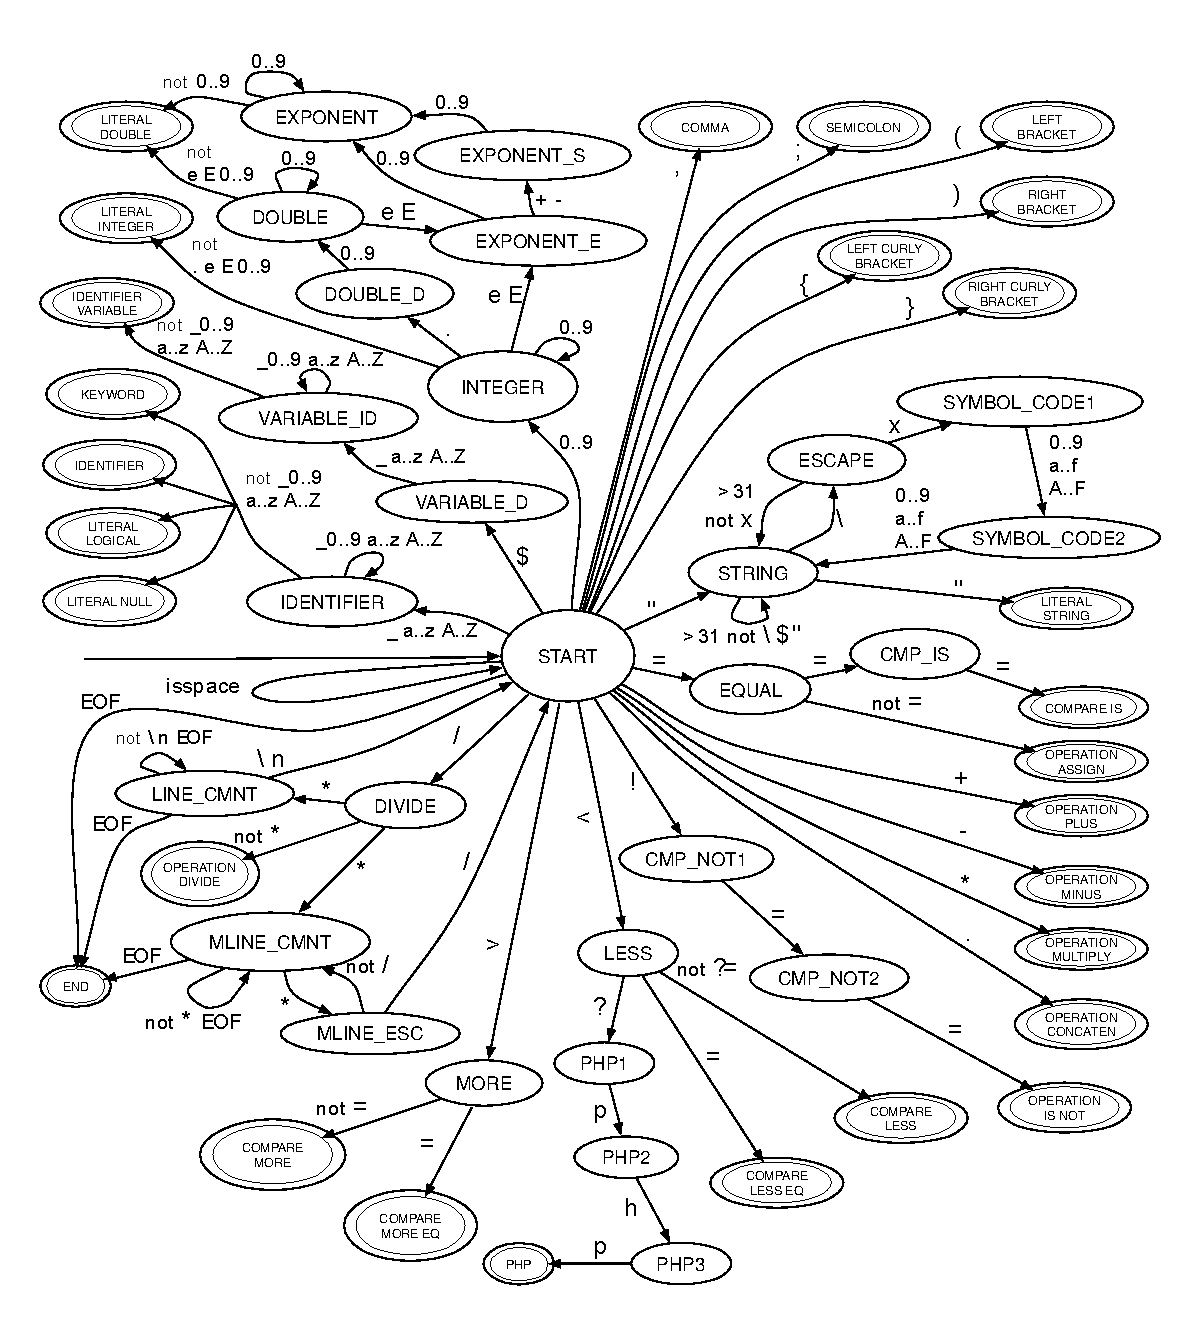
\includegraphics{img/fsm.eps}} 
		\bigskip
		\begin{Large} 
			Slouží pro lexikální analýzu
		\end{Large}
	\end{center}          
		
	\newpage	
	
	

		\subsection{LL-gramatika}
			\begin{center}
  		\begin{tabular}{c l c l} 
				 	1&\textbf{$<$program$>$} & $\rightarrow$ & PHP $\rightarrow$ $<?$php \\ 
				 	& & & \\ 
					2&\textbf{$<$program$\_$units$>$}   &   	$\rightarrow$      &     \emph{$<$func$\_$define$>$ $<$program$\_$units$>$}  \\ 
					3&\textbf{$<$program$\_$units$>$}   &   	$\rightarrow$      &     \emph{$<$cmd$\_$sequence$>$ $<$program$\_$units$>$} \\  
					4&\textbf{$<$program$\_$units$>$}   &    	$\rightarrow$      &     EOF      \\  
 				  & & & \\ 
					5&\textbf{$<$func$\_$define$>$}     &  		$\rightarrow$      &     function id ( \emph{$<$params$>$} ) \{ \emph{$<$cmd$\_$sequence$>$} \} \\ 
					& & & \\ 
					6&\textbf{$<$params$>$}           &    	$\rightarrow$      &     $\varepsilon$\\                                         
					7&\textbf{$<$params$>$}           &      	$\rightarrow$      &     \textdollar id \emph{$<$params$\_$more$>$ } \\ 
	  			& & &  \\ 
					8&\textbf{$<$params$\_$more$>$}     &   		$\rightarrow$      &     , \textdollar id \emph{$<$params$\_$more$>$} \\ 
					9&\textbf{$<$params$\_$more$>$}     &   		$\rightarrow$      &     $\varepsilon$   \\                     
					& & & \\ 
					10&\textbf{$<$cmd$\_$sequence$>$} 	 &   		$\rightarrow$      &     $\varepsilon$     \\                       
					11&\textbf{$<$cmd\_sequence$>$}    &   		$\rightarrow$      &     \emph{$<$cmd$>$ $<$cmd$\_$sequence$>$}  \\ 
 	 				& & &  \\ 
					12&\textbf{$<$cmd$>$}             &       $\rightarrow$      &     \textdollar id = \emph{$<$expression$>$} ;\\ 
					13&\textbf{$<$cmd$>$}             &    $\rightarrow$      &     \textbf{if} ( \emph{$<$expression$>$} ) \{ \emph{$<$cmd$\_$sequence$>$} \} \textbf{else} \{ \emph{$<$cmd$\_$sequence$>$} \} \\        	
					14&\textbf{$<$cmd$>$}             &      $\rightarrow$      &     \textbf{while} ( \emph{$<$expression$>$} ) \{ \emph{$<$cmd$\_$sequence$>$} \} \\  
					15&\textbf{$<$cmd$>$}             &      $\rightarrow$      &     \textbf{return} \emph{$<$expression$>$} ;    \\  
					16&\textbf{$<$cmd$>$}             &     	$\rightarrow$      &     \textdollar id = id ( \emph{$<$input$>$} ) ;  \\ 
					& & & \\ 
					17&\textbf{$<$input$>$}           &   	$\rightarrow$      &     $\varepsilon$      \\     
					18&\textbf{$<$input$>$}           &     	$\rightarrow$      &     \emph{$<$expression$>$ $<$input$\_$more$>$}  \\ 
	 				& & & \\                                                  
					18&\textbf{$<$input$\_$more$>$}     &  			$\rightarrow$      &     , \emph{$<$expression$>$ $<$input$\_$more$>$}  \\  
					19&\textbf{$<$input$\_$more$>$}     &  			$\rightarrow$      &     $\varepsilon$   \\                                             
				\end{tabular}
				\end{center}
	     \centering
			 \bigskip
				\bigskip
			\begin{Large} 
			Slouží pro rekurzivní sestup
			\end{Large}
		

\end{document}
